%%%%%%%%%%%%%%%%%%%%%%%%%%%%%%%%%%%%%%%%%
% Jacobs Landscape Poster
% LaTeX Template
% Version 1.1 (14/06/14)
%
% Created by:
% Computational Physics and Biophysics Group, Jacobs University
% https://teamwork.jacobs-university.de:8443/confluence/display/CoPandBiG/LaTeX+Poster
% 
% Further modified by:
% Nathaniel Johnston (nathaniel@njohnston.ca)
%
% This template has been downloaded from:
% http://www.LaTeXTemplates.com
%
% License:
% CC BY-NC-SA 3.0 (http://creativecommons.org/licenses/by-nc-sa/3.0/)
%
%%%%%%%%%%%%%%%%%%%%%%%%%%%%%%%%%%%%%%%%%


%------------------------------------------------------------------------------
%	PACKAGES AND OTHER DOCUMENT CONFIGURATIONS
%------------------------------------------------------------------------------

\documentclass[final]{beamer}

\usepackage[scale=1.15]{beamerposter} % Use the beamerposter package for laying out the poster
\usepackage{subfig}
\usepackage{multirow}

\usetheme{confposter} % Use the confposter theme supplied with this template

\setbeamercolor{block title}{fg=ngreen!83,bg=white} % Colors of the block titles
\setbeamercolor{block body}{fg=black,bg=white} % Colors of the body of blocks
\setbeamercolor{block alerted title}{fg=white,bg=ngreen!70} % Colors of the highlighted block titles
\setbeamercolor{block alerted body}{fg=black,bg=ngreen!10} % Colors of the body of highlighted blocks
% Many more colors are available for use in beamerthemeconfposter.sty

% Use more stuff from tikz
\usetikzlibrary{arrows, backgrounds, positioning, fit}
\newcommand{\arclen}     {1.5cm}
\newcommand{\nodesize}   {1.8cm}
\newcommand{\nodepad}    {5pt}
\newcommand{\platepad}   {13pt}
\newcommand{\arcwidth}   {3pt}
\newcommand{\fieldwidth} {6pt}
\newcommand{\pointsize}  {4mm}

%-----------------------------------------------------------
% Define the column widths and overall poster size
% To set effective sepwid, onecolwid and twocolwid values, first choose how many columns you want and how much separation you want between columns
% In this template, the separation width chosen is 0.024 of the paper width and a 4-column layout
% onecolwid should therefore be (1-(# of columns+1)*sepwid)/# of columns e.g. (1-(4+1)*0.024)/4 = 0.22
% Set twocolwid to be (2*onecolwid)+sepwid = 0.464
% Set threecolwid to be (3*onecolwid)+2*sepwid = 0.708

\newlength{\sepwid}
\newlength{\onecolwid}
\newlength{\twocolwid}
\newlength{\threecolwid}
\setlength{\paperwidth}{48in} % A0 width: 46.8in
\setlength{\paperheight}{36in} % A0 height: 33.1in
\setlength{\sepwid}{0.024\paperwidth} % Separation width (white space) between columns
\setlength{\onecolwid}{0.22\paperwidth} % Width of one column
\setlength{\twocolwid}{0.464\paperwidth} % Width of two columns
\setlength{\threecolwid}{0.708\paperwidth} % Width of three columns
\setlength{\topmargin}{-0.5in} % Reduce the top margin size
%-----------------------------------------------------------

\usepackage{graphicx}  % Required for including images
\usepackage{booktabs} % Top and bottom rules for tables

% Variables and math notation
%% Define bracket commands (normal, square and curly).
\newcommand{\brac} [1]  {\ensuremath{\left({#1}\right)}}
\newcommand{\sbrac}[1]  {\ensuremath{\left[{#1}\right]}}
\newcommand{\cbrac}[1]  {\ensuremath{\left\{{#1}\right\}}}
\newcommand{\abrac}[1]  {\ensuremath{\left\langle{#1}\right\rangle}}


%% Symbols

% General
\newcommand{\test}       {\ensuremath{^{*}}}
\newcommand{\testT}      {\ensuremath{^{*\top}\!}}
\newcommand{\ttest}      {\ensuremath{^{**}}}
\newcommand{\real}  [1] {\ensuremath{\mathbb{R}^{#1}}}
\newcommand{\ident} [1] {\ensuremath{\mathbf{I}_{#1}}}

% Variables
\newcommand{\lstate}    {\ensuremath{\mathbf{f}}}
\newcommand{\lcov}      {\ensuremath{\boldsymbol{\Sigma}}}
\newcommand{\obs}       {\ensuremath{\mathbf{y}}}
\newcommand{\hyper}     {\ensuremath{\boldsymbol{\theta}}}
\newcommand{\prmean}    {\ensuremath{\boldsymbol{\mu}}}
\newcommand{\prcov}     {\ensuremath{\mathbf{K}}}
\newcommand{\pomean}    {\ensuremath{\mathbf{m}}}
\newcommand{\pocov}     {\ensuremath{\mathbf{C}}}
\newcommand{\xcov}      {\ensuremath{\boldsymbol\Gamma_{\obs\pomean}}}
\newcommand{\Sobs}      {\ensuremath{\mathcal{Y}}}
\newcommand{\Sfunc}     {\ensuremath{\mathcal{M}}}
\newcommand{\scoef}     {\ensuremath{\kappa}}
\newcommand{\Sw}        {\ensuremath{w}}
\newcommand{\Kgain}     {\ensuremath{\mathbf{H}}}
\newcommand{\Linmat}    {\ensuremath{\mathbf{A}}}
\newcommand{\intcpt}    {\ensuremath{\mathbf{b}}}
\newcommand{\Fengy}     {\ensuremath{\mathcal{F}}}
\newcommand{\step}      {\ensuremath{\alpha}}
\newcommand{\jacob}[1]  {\ensuremath{\mathbf{J}_{#1}}}

% Augmented systems
\newcommand{\augobs}    {\ensuremath{\mathbf{z}}}
\newcommand{\augcov}    {\ensuremath{\mathbf{S}}}
\newcommand{\augLinmat} {\ensuremath{\mathbf{B}}}
\newcommand{\augintcpt} {\ensuremath{\mathbf{c}}}

% Gaussian Process
\newcommand{\obss}      {\ensuremath{y}}
\newcommand{\lstates}   {\ensuremath{f}}
\newcommand{\Lins}      {\ensuremath{a}}
\newcommand{\Linvec}    {\ensuremath{\mathbf{a}}}
\newcommand{\intcpts}   {\ensuremath{b}}
\newcommand{\inobs}     {\ensuremath{\mathbf{x}}}
\newcommand{\kernl}     {\ensuremath{k}}
\newcommand{\Kernl}     {\ensuremath{\mathbf{k}}}
\newcommand{\KERNL}     {\ensuremath{\mathbf{K}}}
\newcommand{\lvar}      {\ensuremath{\sigma^2}}
\newcommand{\lstd}      {\ensuremath{\sigma}}
\newcommand{\Lvar}      {\ensuremath{\boldsymbol\Lambda}}
\newcommand{\pomeans}   {\ensuremath{m}}
\newcommand{\pocovs}    {\ensuremath{C}}
\newcommand{\xcovs}     {\ensuremath{\Gamma}}
\newcommand{\khyper}    {\ensuremath{\theta}}
\newcommand{\khypers}   {\ensuremath{\boldsymbol\theta}}


%% Operations
\newcommand{\transpose}  {\ensuremath{^{\!\top}}}
\newcommand{\inv}        {\ensuremath{^{\text{-}1}}}
\newcommand{\deter}[1]   {\ensuremath{\left|{#1}\right|}}
\newcommand{\trace}[1]   {\ensuremath{\text{tr}\!\brac{#1}}}
\newcommand{\diag}[1]    {\ensuremath{\text{diag}\!\brac{#1}}}
\newcommand{\expec}[2]   {\ensuremath{\abrac{#2}_{\!{#1}}}}
\newcommand{\expece}[2]  {\ensuremath{\mathbb{E}_{#1}\!\sbrac{#2}}}
\newcommand{\evar} [2]   {\ensuremath{\mathbb{V}_{#1}\!\sbrac{#2}}}
\newcommand{\KL}[2]      {\ensuremath{\text{KL}\!\sbrac{{#1}\!\parallel\!{#2}}}}
\newcommand{\entropy}[1] {\ensuremath{\mathbb{H}\sbrac{#1}}}
\newcommand{\lnorm}[2]   {\ensuremath{\left\|{#2}\right\|_{{#1}}}}


%% Functions, PDFs etc
\newcommand{\nonlin}[1] {\ensuremath{g\!\brac{{#1}}}}
\newcommand{\augnonlin}[1] {\ensuremath{h\!\brac{{#1}}}}
\newcommand{\prob}  [1] {\ensuremath{p\!\brac{#1}}}
\newcommand{\probC} [2] {\ensuremath{p\!\left({#1}\middle\vert{#2}\right)}}
\newcommand{\qrob}  [1] {\ensuremath{q\!\brac{#1}}}
\newcommand{\qrobC} [2] {\ensuremath{q\!\left({#1}\middle\vert{#2}\right)}}
\newcommand{\gaus}  [1] {\ensuremath{\mathcal{N}\!\brac{#1}}}
\newcommand{\gausC} [2] {\ensuremath{\mathcal{N}\!\left({#1}\middle\vert{#2}\right)}}
\newcommand{\bern}  [1] {\ensuremath{\textrm{Bern}\!\brac{#1}}}
\newcommand{\bernC} [2] {\ensuremath{\textrm{Bern}\!\left({#1}\middle\vert{#2}\right)}}
\newcommand{\kfunc} [2] {\ensuremath{\kernl\!\brac{{#1}, {#2}}}}
\newcommand{\expon} [2] {\ensuremath{{#1}\!\times\!10^{#2}}}


%% Operators
\DeclareMathOperator*{\argmax}{\operatorname*{argmax}}
\DeclareMathOperator*{\argmin}{\operatorname*{argmin}}


% Red underline
\newsavebox\MBox
\newcommand\Cline[2][red]{{\sbox\MBox{$#2$}%
  \rlap{\usebox\MBox}\color{#1}\rule[-1.6\dp\MBox]{\wd\MBox}{0.7pt}}}


%------------------------------------------------------------------------------
%	TITLE SECTION 
%------------------------------------------------------------------------------

\title{Extended and Unscented Gaussian Processes} % Poster title

\author{Daniel M.\ Steinberg\textsuperscript{1} 
        \texttt{\small(daniel.steinberg@nicta.com.au)} and
        Edwin V.\ Bonilla\textsuperscript{2}
        \texttt{\small(e.bonilla@unsw.edu.au)}} % Author(s)

\institute{\textsuperscript{1}NICTA, 
           \textsuperscript{2}The University of New South Wales} % Institution(s)

%------------------------------------------------------------------------------

\begin{document}

\addtobeamertemplate{block end}{}{\vspace*{2ex}} % White space under blocks
\addtobeamertemplate{block alerted end}{}{\vspace*{2ex}} % White space under highlighted (alert) blocks

%\setlength{\belowcaptionskip}{2ex} % White space under figures
%\setlength\belowdisplayshortskip{2ex} % White space under equations

\begin{frame}[t] % The whole poster is enclosed in one beamer frame

\begin{columns}[t] % The whole poster consists of three major columns, the second of which is split into two columns twice - the [t] option aligns each column's content to the top

\begin{column}{\sepwid}\end{column} % Empty spacer column

\begin{column}{\onecolwid} % The first column


%------------------------------------------------------------------------------
%	Problem statement and aims
%------------------------------------------------------------------------------

\begin{alertblock}{Inverse Problems}

Many problems in science and engineering have some \textbf{forward} or system
model, $\nonlin{\cdot}$, which is often nonlinear:
\begin{equation*}
    \obs = \nonlin{\lstate} + \boldsymbol\epsilon
\end{equation*}
\vspace{-2cm}
\begin{itemize}
    \item We can measure the outputs of the system, $\obs$, but the inputs,
        $\lstate$, are \textbf{latent}.
    \item We wish to infer these inputs \emph{without} access to the inverse
        system model, $\nonlininv{\cdot}$.
    \item $\obs$ may be a continuous process or path (robot arm motion), 
        so $\lstate$ is a \textbf{Gaussian Process}.
\end{itemize}

\end{alertblock}


\begin{block}{Aims}

\begin{enumerate}
    \item We require a posterior distribution over $\lstate$.
    \item We don't want to re-derive the
        learning equations for every new $\nonlin{\cdot}$.
    \item The gradients, $\partial{\nonlin{\lstate}} /
        \partial\lstate$, may not be known.
    \item Learning has to be fast (not MCMC).
\end{enumerate}

\end{block}


%------------------------------------------------------------------------------
%	INTRODUCTION
%------------------------------------------------------------------------------

\begin{block}{GPs with nonlinear likelihoods}

Prior on latent functions $\lstate$ at inputs $\Inobs =
\cbrac{\inobs_n}^N_{n=1}$,
\begin{equation}
    \prob{\lstate} = \gausC{\lstate}{\mathbf{0}, \KERNL\!\brac{\Inobs, \Inobs}}
\end{equation}
Likelihood -- encodes $\obs = \nonlin{\lstate} + \boldsymbol{\epsilon}$,
\begin{equation}
    \probC{\obs}{\lstate}
    = \gausC{\obs}{\Cline{\nonlin{\lstate}}, \lvar\ident{N}}
    = \prod_{n=1}^N 
        \gausC{\obss_n}{\Cline{\nonlin{\lstates_n}}, \lvar}
    \label{eq:like}
\end{equation}%
Inverse solution is the posterior,
\begin{equation}
    \probC{\lstate}{\obs} = \frac{\probC{\obs}{\lstate}\prob{\lstate}}
        {\prob{\obs}}
    \label{eq:post}
\end{equation}
But the marginal likelihood is intractable,
\begin{equation}
    \prob{\obs} = \int \gausC{\obs}{\Cline{\nonlin{\lstate}}, \lvar\ident{N}}
        \gausC{\lstate}{\mathbf{0}, \KERNL} d\lstate
\end{equation}

\end{block}


%------------------------------------------------------------------------------
%	Nonlinear Gaussian Models
%------------------------------------------------------------------------------

%\vspace{-1.5cm}
\begin{figure}
    %\subfloat[][]{
        %\vspace{-2cm}
        %\pgfdeclarelayer{Ilayer}
\pgfsetlayers{Ilayer,main}
%
\begin{tikzpicture}
    [	
	    font=\small, 
		node distance=1.5cm,
		odist/.style ={circle, draw=black!60, thick, inner sep=5pt, 
                        minimum size=1cm, fill=black!25},
		pdist/.style ={circle, draw=black!60, dashed, thick, inner sep=5pt, 
                        minimum size=1cm, fill=black!25},
		dist/.style  ={circle, draw=black!60, thick, inner sep=5pt, 
                        minimum size=1cm},
		point/.style ={circle,draw=black!60,fill=black!60,thick,inner sep=0pt,
                       minimum size=2mm},
		oarc/.style  ={->,>=latex',thick},
		plate/.style ={draw=black!60,rounded corners,thick,inner sep=13pt},
		reps/.style  ={anchor=south east,inner sep=3pt}
	]

    \node[dist]     (q0)                         {$\lstate$};

    \node[point]    (mean)  [above=of q0,xshift=-1cm,label=$\prmean$] {};

    \node[point]    (cov)   [above=of q0,xshift=1cm,label=$\prcov$]  {};

    \node[odist]    (x0)    [below=of q0]        {$\obs$};

    \node[point]    (lcov)  [right=of x0,label=$\lcov$]  {};

    \draw[oarc]     (q0) to (x0);
    \draw[oarc]     (mean) to (q0);
    \draw[oarc]     (cov) to (q0);
    \draw[oarc]     (lcov) to (x0);
    
\end{tikzpicture}

        %\label{sfig:gaus}
    %}
    %\subfloat[][]{
        %
\pgfdeclarelayer{Ilayer}
\pgfsetlayers{Ilayer,main}
%
\begin{tikzpicture}
    [	
	    font=\footnotesize, 
		node distance=5mm,
		odist/.style ={circle, draw=black!60, thick, inner sep=1pt, 
                        minimum size=6mm, fill=black!25},
		pdist/.style ={circle, draw=black!60, dashed, thick, inner sep=1pt, 
                        minimum size=6mm, fill=black!25},
		dist/.style  ={circle, draw=black!60, thick, inner sep=1pt, 
                        minimum size=6mm},
		point/.style ={circle,draw=black!60,fill=black!60,thick,inner sep=0pt,
                       minimum size=2mm},
		oarc/.style  ={->,>=latex',thick},
		ofeild/.style  ={-,>=latex',line width=0.8mm},
		plate/.style ={draw=black!60,rounded corners,thick,inner sep=13pt},
		reps/.style  ={anchor=south east,inner sep=3pt}
	]

    
    \node[dist]     (q0)                         {$\lstates_0$};
    \node[dist]     (q1)    [right=of q0]        {$\lstates_1$};
    \node[dist]     (q2)    [right=of q1]        {$\lstates_2$};
    \node[dist]     (q3)    [right=of q2]        {$\lstates_3$};
    \node           (d2)    [right=of q3]        {$\ldots$};

    \node[point]     (i0)    [above=of q0, label=$\inobs_0$]    {};
    \node[point]     (i1)    [above=of q1, label=$\inobs_1$]    {};
    \node[point]     (i2)    [above=of q2, label=$\inobs_2$]    {};
    \node[point]     (i3)    [above=of q3, label=$\inobs_3$]    {};
    \node            (d1)    [above=of d2, yshift=4mm]          {$\ldots$};

    \node[odist]    (x0)    [below=of q0]        {$\obss_{0}$};
    \node[odist]    (x1)    [right=of x0]        {$\obss_{1}$};
    \node[odist]    (x2)    [right=of x1]        {$\obss_{2}$};
    \node[odist]    (x3)    [right=of x2]        {$\obss_{3}$};
    \node           (d3)    [right=of x3]        {$\ldots$};
    
    \node[point]    (lcov)  [below=of x1,xshift=5mm,label=below:$\lstd$] {};

    \draw[ofeild]     (q0) to (q1);
    \draw[ofeild]     (q1) to (q2);
    \draw[ofeild]     (q2) to (q3);
    \draw[ofeild]     (q3) to (d2);

    \draw[oarc]     (i0) to (q0);
    \draw[oarc]     (i1) to (q1);
    \draw[oarc]     (i2) to (q2);
    \draw[oarc]     (i3) to (q3);

    \draw[oarc]     (q0) to (x0);
    \draw[oarc]     (q1) to (x1);
    \draw[oarc]     (q2) to (x2);
    \draw[oarc]     (q3) to (x3);

    \draw[oarc]     (lcov) to (x0);
    \draw[oarc]     (lcov) to (x1);
    \draw[oarc]     (lcov) to (x2);
    \draw[oarc]     (lcov) to (x3);
    
\end{tikzpicture}


        %\label{sfig:gp}
    %}
    %\caption{Graphical model of nonlinear Gaussian \subref{sfig:gaus} and
        %Gaussian process \subref{sfig:gp} inversion problems.}

    
\pgfdeclarelayer{Ilayer}
\pgfsetlayers{Ilayer,main}
%
\begin{tikzpicture}
    [	
	    font=\footnotesize, 
		node distance=5mm,
		odist/.style ={circle, draw=black!60, thick, inner sep=1pt, 
                        minimum size=6mm, fill=black!25},
		pdist/.style ={circle, draw=black!60, dashed, thick, inner sep=1pt, 
                        minimum size=6mm, fill=black!25},
		dist/.style  ={circle, draw=black!60, thick, inner sep=1pt, 
                        minimum size=6mm},
		point/.style ={circle,draw=black!60,fill=black!60,thick,inner sep=0pt,
                       minimum size=2mm},
		oarc/.style  ={->,>=latex',thick},
		ofeild/.style  ={-,>=latex',line width=0.8mm},
		plate/.style ={draw=black!60,rounded corners,thick,inner sep=13pt},
		reps/.style  ={anchor=south east,inner sep=3pt}
	]

    
    \node[dist]     (q0)                         {$\lstates_0$};
    \node[dist]     (q1)    [right=of q0]        {$\lstates_1$};
    \node[dist]     (q2)    [right=of q1]        {$\lstates_2$};
    \node[dist]     (q3)    [right=of q2]        {$\lstates_3$};
    \node           (d2)    [right=of q3]        {$\ldots$};

    \node[point]     (i0)    [above=of q0, label=$\inobs_0$]    {};
    \node[point]     (i1)    [above=of q1, label=$\inobs_1$]    {};
    \node[point]     (i2)    [above=of q2, label=$\inobs_2$]    {};
    \node[point]     (i3)    [above=of q3, label=$\inobs_3$]    {};
    \node            (d1)    [above=of d2, yshift=4mm]          {$\ldots$};

    \node[odist]    (x0)    [below=of q0]        {$\obss_{0}$};
    \node[odist]    (x1)    [right=of x0]        {$\obss_{1}$};
    \node[odist]    (x2)    [right=of x1]        {$\obss_{2}$};
    \node[odist]    (x3)    [right=of x2]        {$\obss_{3}$};
    \node           (d3)    [right=of x3]        {$\ldots$};
    
    \node[point]    (lcov)  [below=of x1,xshift=5mm,label=below:$\lstd$] {};

    \draw[ofeild]     (q0) to (q1);
    \draw[ofeild]     (q1) to (q2);
    \draw[ofeild]     (q2) to (q3);
    \draw[ofeild]     (q3) to (d2);

    \draw[oarc]     (i0) to (q0);
    \draw[oarc]     (i1) to (q1);
    \draw[oarc]     (i2) to (q2);
    \draw[oarc]     (i3) to (q3);

    \draw[oarc]     (q0) to (x0);
    \draw[oarc]     (q1) to (x1);
    \draw[oarc]     (q2) to (x2);
    \draw[oarc]     (q3) to (x3);

    \draw[oarc]     (lcov) to (x0);
    \draw[oarc]     (lcov) to (x1);
    \draw[oarc]     (lcov) to (x2);
    \draw[oarc]     (lcov) to (x3);
    
\end{tikzpicture}


    \label{fig:gp}

    \caption{A Gaussian process for inversion problems -- the mapping from the
        distribution over $\lstates_n$ to $\obss_n$ is nonlinear.}
\end{figure}


%----------------------------------------------------------------------------------------

\end{column} % End of the first column

\begin{column}{\sepwid}\end{column} % Empty spacer column

\begin{column}{\twocolwid} % Begin a column which is two columns wide (column 2)

\begin{columns}[t,totalwidth=\twocolwid] % Split up the two columns wide column

\begin{column}{\onecolwid}\vspace{-.6in} % The first column within column 2 (column 2.1)


%------------------------------------------------------------------------------
%	Inference and Linearization
%------------------------------------------------------------------------------

\begin{block}{Variational Inference}

In variational inference we can \emph{approximate} the posterior,
$\probC{\lstate}{\obs} \approx \qrob{\lstate} = \gausC{\lstate} {\pomean,
    \pocov}$, and then establish as \emph{lower bound} on the log marginal
likelihood,
\begin{equation}
    \Fengy = \expec{q\lstate}{\log \probC{\obs}{\lstate}}
        - \KL{\qrob{\lstate}}{\prob{\lstate}}.
    \label{eq:fengy}
\end{equation}
Then we use $\Fengy$ to \emph{optimise} posterior parameters:
\begin{equation}
    \pomean^* = \argmax_\pomean{\Fengy}, \qquad
    \pocov^* = \argmax_\pocov{\Fengy},
\end{equation}
where $\qrob{\lstate}$ should approach the true posterior
$\probC{\lstate}{\obs}$. \emph{But}, the expected log likelihood has an
intractable quadratic term,
\begin{equation*}
    \expec{q\lstate}{\log \probC{\obs}{\lstate}} = 
    -\frac{1}{2\lvar} \expec{q\lstate}{
        \brac{\obs - \Cline{\nonlin{\lstate}}}\transpose
        \brac{\obs - \Cline{\nonlin{\lstate}}}} + \ldots
\end{equation*}
We use two tricks to get around this problem;
\begin{enumerate}
    \item \textbf{linearize} the forward model $\nonlin{\lstate}$,
        \begin{equation}
            \nonlin{\lstate} \approx \Linmat\lstate + \intcpt
            \label{eq:linearize}
        \end{equation}
    \item \textbf{Newton method} and linearized $\tilde\Fengy$ to
        find~$\pomean$,
        \begin{equation}
            \pomean_{k+1} = \pomean_k -
            \step\brac{\nabla_\pomean\nabla_\pomean\tilde\Fengy}\inv 
                \nabla_\pomean\tilde\Fengy
            \label{eq:newton}
        \end{equation}
\end{enumerate}
Then $\pocov$ is found by maximising $\tilde\Fengy$.

%Posterion parameters:
%\begin{align}
    %\pomean_{k+1} &= \brac{1-\step}\pomean_k + \step\prmean 
        %+ \step\Kgain_k\brac{\obs - \intcpt_k - \Linmat_k\prmean},
        %\label{eq:pomean} \\
    %\Kgain_k &= \prcov\Linmat_k\transpose\brac{\lcov +
        %\Linmat_k\prcov\Linmat_k\transpose}\inv, 
        %\label{eq:kgain} \\
    %\pocov &= \brac{\ident{D} - \Kgain\Linmat}\!\prcov
    %\label{eq:pocov}
%\end{align}

\end{block}

%----------------------------------------------------------------------------------------

\end{column} % End of column 2.1

\begin{column}{\onecolwid}\vspace{-.6in} % The second column within column 2 (column 2.2)

%----------------------------------------------------------------------------------------
%	METHODS
%----------------------------------------------------------------------------------------

\begin{block}{EGP -- Taylor Series Linearization}
    
\begin{figure}
    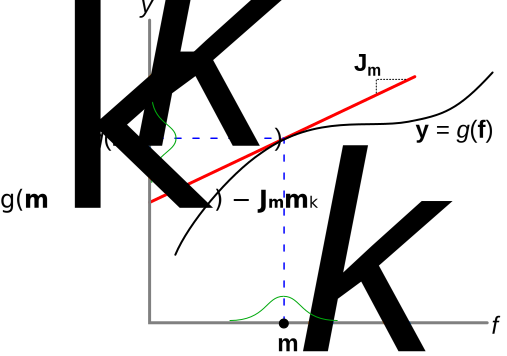
\includegraphics[height=14cm]{fig/taylor}
    \hspace{3cm}
    \caption{Demonstration of linearizing the forward model, $\nonlin{\cdot}$
        using a first order Taylor series expansion.}
\end{figure}        

First order Taylor series expansion about $\pomean_k$,
\begin{equation*}
    \nonlin{\lstate} \approx \nonlin{\pomean_k} +
    \jacob{\pomean_k}\brac{\lstate - \pomean_k},
\end{equation*}
here $\jacob{\pomean_k}$ = $\partial\nonlin{\pomean_k}\!/
\partial\pomean_k$. Then equating coefficients gives,
\begin{equation}
    \Linmat = \jacob{\pomean_k} \quad \text{and} \quad
    \intcpt = \nonlin{\pomean_k} - \jacob{\pomean_k}\pomean_k.
\end{equation}
This results in the \emph{Gauss Newton} method.

\end{block}

%----------------------------------------------------------------------------------------

\end{column} % End of column 2.2

\end{columns} % End of the split of column 2 - any content after this will now take up 2 columns width

%----------------------------------------------------------------------------------------
%	IMPORTANT RESULT
%----------------------------------------------------------------------------------------

\begin{alertblock}{Key Results}

\begin{itemize}

    \item The unscented Gaussian process does not require any gradients
        $\partial\nonlin{\lstate}\!/\partial\lstate$ to learn the posterior.

    \item $\Linmat = \diag{\Lins_0, \ldots, \Lins_N}$ from the factorising
        likelihood \eqref{eq:like}. Similar complexity as Laplace
        approximation.

    \item We can also derive the iterative extended and sigma-point Kalman
        filters using this framework.
\end{itemize}

\end{alertblock} 

%------------------------------------------------------------------------------

\vspace{-1.5cm}


\begin{columns}[t,totalwidth=\twocolwid] % Split up the two columns wide column again

%\begin{column}{\onecolwid} % the first column within column 2 (column 2.1)
\begin{column}{\twocolwid}


\begin{block}{Experiments}

\begin{columns}
\begin{column}{0.38\twocolwid}

\textbf{Toy inversion problems} -- something about this experiment...

\begin{table}[tb]
    \centering
    \caption[]{The nonlinear GPs with various differentiable nonlinear functions.}
    \tiny
    \begin{tabular}{r|c| c c c c c c}
        \multirow{2}{*}{$\nonlin{\lstate}$} & \multirow{2}{*}{Algorithm} & 
            \multicolumn{2}{c}{NLPD $\lstates\test$} &
            \multicolumn{2}{c}{SMSE $\lstates\test$} &
            \multicolumn{2}{c}{SMSE $\obss\test$} \\
        & & mean & std. & mean & std. & mean & std.\\
        \toprule
        $\lstate$ 
& UGP & -0.90046 & 0.06743 & 0.01219 & 0.00171 & -- & -- \\
& EGP & -0.89908 & 0.06608 & 0.01224 & 0.00178 & -- & -- \\
& \cite{Opper2009} & -0.27590 & 0.06884 & 0.01249 & 0.00159 & -- & -- \\
& GP & \textbf{-0.90278} & 0.06988 & \textbf{0.01211} & 0.00160 & -- & -- \\
        \midrule
        $\lstate^3 + \lstate^2 + \lstate$ 
& UGP & \textbf{-0.23622} & 1.72609 & 0.01534 & 0.00202 & \textbf{0.02184} & 0.00525 \\
& EGP & -0.22325 & 1.76231 & \textbf{0.01518} & 0.00203 & \textbf{0.02184} & 0.00528 \\
& \cite{Opper2009} & -0.14559 & 0.04026 & 0.06733 & 0.01421 & 0.02686 & 0.00266 \\
        \midrule
        $\exp\!\brac{\lstate}$ 
& UGP & -0.75475 & 0.32376 & \textbf{0.13860} & 0.04833 & \textbf{0.03865} & 0.00403 \\
& EGP & \textbf{-0.75706} & 0.32051 & 0.13971 & 0.04842 & 0.03872 & 0.00411 \\
& \cite{Opper2009} & -0.08176 & 0.10986 & 0.17614 & 0.04845 & 0.05956 & 0.01070 \\
        \midrule
        $\sin\!\brac{\lstate}$ 
& UGP & \textbf{-0.59710} & 0.22861 & \textbf{0.03305} & 0.00840 & 0.11513 & 0.00521 \\
& EGP & -0.59705 & 0.21611 & 0.03480 & 0.00791 & \textbf{0.11478} & 0.00532 \\
& \cite{Opper2009} & -0.04363 & 0.03883 & 0.05913 & 0.01079 & 0.11890 & 0.00652 \\
        \midrule
        $\tanh\!\brac{2\lstate}$
& UGP & \textbf{0.01101} & 0.60256 & \textbf{0.15703} & 0.06077 & \textbf{0.08767} & 0.00292 \\
& EGP & 0.57403 & 1.25248 & 0.18739 & 0.07869 & 0.08874 & 0.00394 \\
& \cite{Opper2009} & 0.15743 & 0.14663 & 0.16049 & 0.04563 & 0.09434 & 0.00425 \\
        \bottomrule
    \end{tabular}
    \label{tab:toy}
\end{table}

\end{column}
\begin{column}{0.29\twocolwid}\vspace{-.8in}

\begin{figure}
    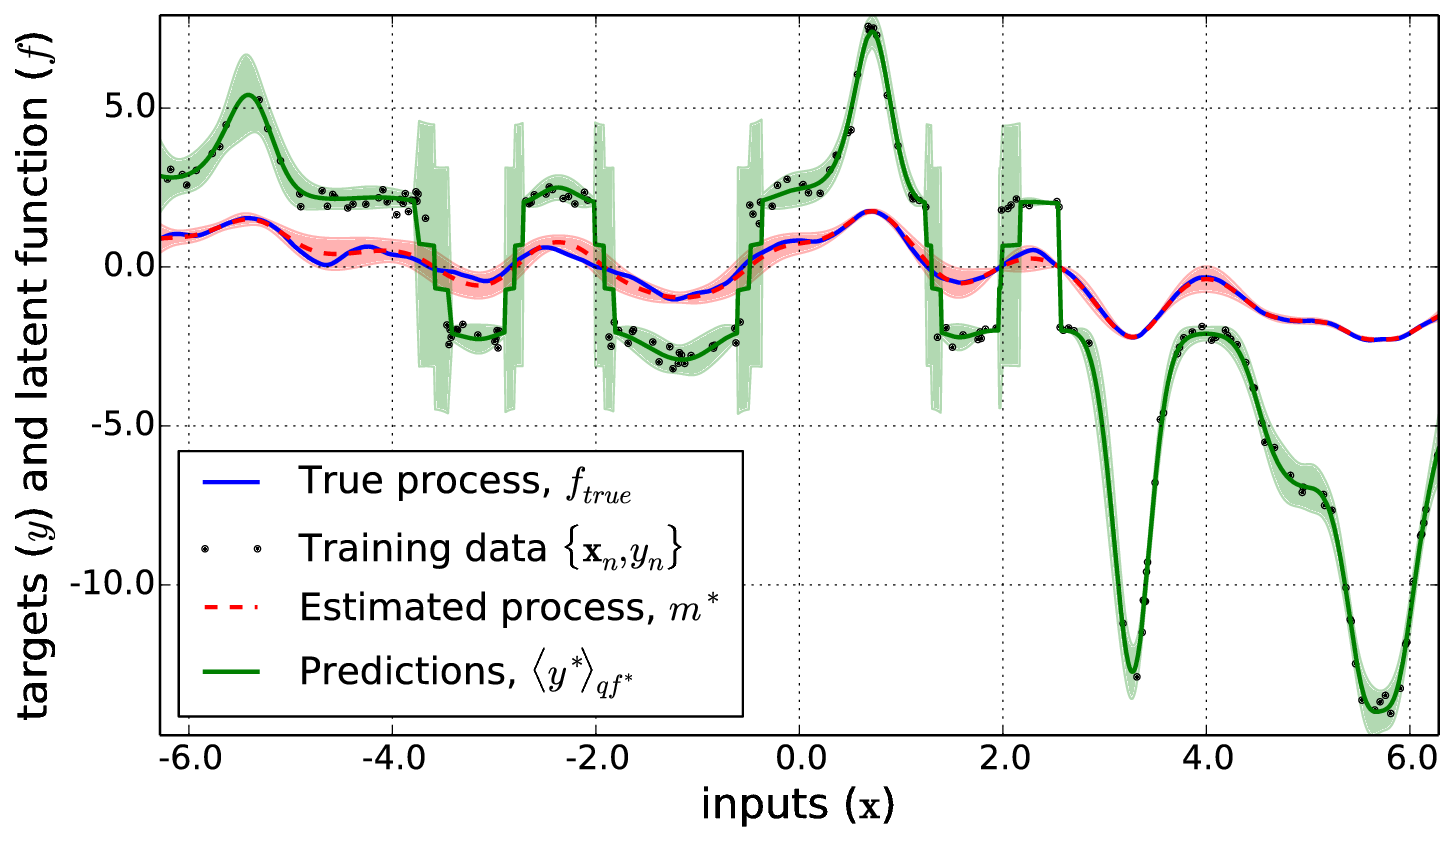
\includegraphics[width=0.6\onecolwid]{fig/signdemo.png}
    \caption[]{Learning the UGP with the forward model, $\nonlin{\lstate} = 
            2\times\text{sign}\!\brac{\lstate} + \lstate^3$. This function does
            not have derivatives at the zero crossing points.}
   \label{fig:sign}
\end{figure}

\end{column}
\begin{column}{0.29\twocolwid}\vspace{-1.8in}

\textbf{Binary classification} -- something about this experiment too ...

\begin{table}[tb]
    \centering
    \caption[]{Classification performance on the USPS handwritten-digits
        dataset for numbers `3' and `5'.}
    \tiny
    \begin{tabular}{r| c c c c}
    Algorithm & NLP $\obss\test$ & Error rate (\%) 
        & $\log\!\brac{\sigma_\text{se}}$ & $\log\!\brac{l_\text{se}}$ \\
    \toprule
    GP -- Laplace & 0.11528 & 2.9754 & 2.5855 & 2.5823 \\
    GP -- EP & 0.07522 & 2.4580 & 5.2209 & 2.5315 \\
    GP -- VB & 0.10891 & 3.3635 & 0.9045 & 2.0664 \\ 
    SVM (RBF) & 0.08055 & 2.3286 & -- & -- \\
    Logistic Reg. & 0.11995 & 3.6223 & -- & -- \\
    \midrule
    UGP & \textbf{0.07290} & \textbf{1.9405} & 1.5743 & 1.5262 \\
    EGP & 0.08051 & 2.1992 & 2.9134 & 1.7872 \\
    %UGP & 0.06524 & 2.1992 & 1.5140 & 1.4257 \\
    %EGP & 0.12946 & 2.0699 & 3.3068 & 1.7480 \\
    \bottomrule
    \end{tabular}
    \label{tab:class}
\end{table}

\vfill

\end{column}
\end{columns}
\end{block}


\end{column} % End of column 2.1

%\begin{column}{\onecolwid} % The second column within column 2 (column 2.2)



%\begin{block}{Experiments}

%\end{block}


%----------------------------------------------------------------------------------------

%\end{column} % End of column 2.2

\end{columns} % End of the split of column 2

\end{column} % End of the second column

\begin{column}{\sepwid}\end{column} % Empty spacer column

\begin{column}{\onecolwid} % The third column

%----------------------------------------------------------------------------------------

\begin{block}{UGP -- Unscented Transform}

\begin{figure}
    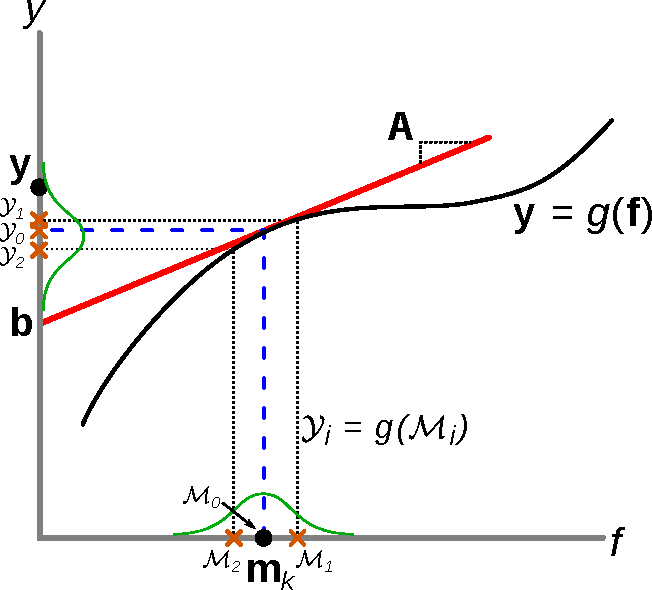
\includegraphics[height=14cm]{fig/statlin}
    \caption{Demonstration of linearizing the foward model, $\nonlin{\cdot}$
        using the unscented transform.}
\end{figure}        

Make sigma points \cite{Julier2004, Geist2010}, $\Sfunc_i$ and $\Sobs_i$, then
solving a linear regression problem,
\begin{equation*}
    \argmin_{\Linmat, \intcpt} \sum^{2D}_{i=0} 
        \lnorm{2}{\Sobs_i - \brac{\Linmat\Sfunc_i + \intcpt}}^2
\end{equation*}
gives,
\begin{equation}
    \Linmat = \xcov \pocov\inv \quad \text{and} \quad
    \intcpt = \bar\obs - \Linmat\pomean,
\end{equation}
and $\xcov$ is the cross-covariance between $\Sfunc_i$ and~$\Sobs_i$.

\end{block}


\begin{block}{Kernel Hyperparameters}

Learning the hyperparameters, $\khypers$ in $\kernl\!\brac{\inobs,
    \inobs'|\khypers}$, is usually an optimisation $\khypers^* =
\argmax_{\khypers}\Fengy$,%
\begin{itemize}
    \item but $\pomean$ is an implicit function of $\khypers$,
    \item so $\nabla_{\khypers}\Fengy$ also requires various derivatives of
        $\nonlin{\cdot}$.
\end{itemize}
\emph{Solution}: numerical gradient methods (BOBYQA in NLopt) work well -- for
a few hyperparameters.

\end{block}


%\begin{block}{Conclusion}


%\end{block}

%----------------------------------------------------------------------------------------
%	REFERENCES
%----------------------------------------------------------------------------------------

\begin{block}{References}

%\nocite{*} % Insert publications even if they are not cited in the poster
\small{\bibliographystyle{unsrt}
\bibliography{nips2014lin}\vspace{0.75in}}

\end{block}

%----------------------------------------------------------------------------------------
%	ACKNOWLEDGEMENTS
%----------------------------------------------------------------------------------------

%\setbeamercolor{block title}{fg=red,bg=white} % Change the block title color

%\begin{block}{Acknowledgements}

%\footnotesize{\rmfamily{This research was supported by the Science Industry Endowment
        %Fund (RP 04-174) Big Data Knowledge Discovery project. NICTA is funded
        %by the Australian Government through the Department of Communications
        %and the Australian Research Council through the ICT Centre of
        %Excellence Program.}} \\

%\end{block}


%----------------------------------------------------------------------------------------
%	Additional INFORMATION
%----------------------------------------------------------------------------------------

\setbeamercolor{block alerted title}{fg=white,bg=npurple!62} % Change the alert block title colors
\setbeamercolor{block alerted body}{fg=black,bg=white} % Change the alert block body colors

\vspace{-2cm}
\begin{alertblock}{Code}

Github -- \href{https://github.com/NICTA/linearizedGP}
                 {https://github.com/NICTA/linearizedGP}
\end{alertblock}

%----------------------------------------------------------------------------------------

\end{column} % End of the third column

\end{columns} % End of all the columns in the poster

\end{frame} % End of the enclosing frame

\end{document}


%%% MAYBE TODO:
% - Flesh out experiments captions
% - Make sure the linearization descriptions are 1d, they are not right now!
% - Make the figures demonstrating the linearization more reflective of the GP
%   (i.e. multiple linearization)
% - Add in posterior parameter update equations?
% - Add in prediction equations?
% - Make the equations reflect the 1-D linearizations?
% - Make A and b red to clarify their importance?
